\chapter{Distinguishing Time-Delayed Causal Interactions Using Convergent Cross Mapping}
\label{chap_ccm_time_delays}

\section{Abstract}
An important problem across many scientific fields is the identification of causal effects from observational data alone. Recent methods (convergent cross mapping, CCM) have made substantial progress on this problem by applying the idea of nonlinear attractor reconstruction to time series data. Here, we expand upon the technique of CCM by explicitly considering time lags. Applying this extended method to representative examples (model simulations, a laboratory predator-prey experiment, temperature and greenhouse gas reconstructions from the Vostok ice core, and long-term ecological time series collected in the Southern California Bight), we demonstrate the ability to identify different time-delayed interactions, distinguish between synchrony induced by strong unidirectional-forcing and true bidirectional causality, and resolve transitive causal chains. 

\section{Introduction}

A fundamental question in science is identifying the causal relationships between variables. The conventional approach to this problem is to observe the outcomes of controlled experiments; however, this is not always possible due to moral, legal, or feasibility reasons. Consequently, the ability to infer causality using only observational data is a highly valuable tool with applications in many fields of study (e.g., financial systems, ecosystems, neuroscience \cite{Granger_1969, Hiemstra_1994, Chen_2006, Sugihara_2012}).

Early on, Bishop Berkeley \cite{Berkeley_1710} warned that the co-occurrence of events did not necessarily mean that they are causally related (i.e., correlation does not imply causation). Even so, the use of correlation to suggest causality (or more frequently, the lack of correlation suggesting no causality) has remained a common, heuristic notion, and is still commonly applied today. In 1969, however, Granger \cite{Granger_1969} suggested an alternative framework for detecting causality based on the idea of using prediction as a criterion. In the Granger causality framework, a variable $x$ is said to ``cause'' variable $y$ if $x$ has unique information (i.e., not found in other variables) that can improve the prediction of $y$. Thus, causality could be inferred if the optimal model for $y$ improves when $x$ is included. However, Granger noted that this approach might not apply in dynamic systems, and indeed, Sugihara et al. \cite{Sugihara_2012} showed that it does not: in dynamic systems with behaviors that are at least somewhat deterministic, information about past states is carried forward through time (i.e., the system is not completely stochastic). Thus, Takens' Theorem \cite{Takens_1981} applies, and so if $x$ is indeed causal to $y$, then information about $x$ must be recorded in $y$. Consequently, causal variables (i.e., $x$) cannot contain unique information (it will also be recorded in the affected variables), and so Granger's test is invalid (except in certain cases; see Discussion). 

As an alternative test for causality, Sugihara et al. \cite{Sugihara_2012} suggested a new method, convergent cross mapping (CCM). It follows from Takens' Theorem \cite{Takens_1981} that if $x$ does influence $y$, then the historical values of $x$ can be recovered from variable $y$ alone. In practical terms, this is accomplished using the technique of ``cross mapping'': a time delay embedding is constructed from the time series of $y$, and the ability to estimate the values of $x$ from this embedding quantifies how much information about $x$ has been encoded into $y$. Thus, the causal effect of $x$ on $y$ is determined by how well $y$ cross maps $x$. This approach is described in further detail in the materials and methods, but also summarized in this short instructional animation: (\url{https://www.youtube.com/playlist?list=PL-SSmlAMhY3bnogGTe2tf7hpWpl508pZZ}).

Although CCM can be successfully applied to systems with weak to moderate coupling strengths, Sugihara et al. observed that exceptionally strong unidirectional forcing can lead to the phenomenon of ``generalized synchrony'' \cite{Rulkov_1995}. In these situations, the dynamics of a response variable, $y$, become dominated by those of the driving variable, $x$, such that the full system (consisting of both the response variable and driving variable) collapses to just that of the driving variable. Although there is no causal effect of $y$ on $x$, the states of the driving variable $x$ can uniquely determine the response variable $y$, and so CCM is observed in both directions (i.e., $x$ cross maps $y$ and $y$ cross maps $x$). Thus, CCM appears to be limited by the fact that it may not be able to distinguish between bidirectional causality and strong unidirectional causality that leads to synchrony.

Here, we propose an extension to CCM that can resolve this problem: by explicitly considering different lags for cross mapping, it is possible to determine whether a driving variable acts with some time delay on a response variable. In the case of synchrony caused by strong unidirectional forcing, this approach should detect a negative lag for cross mapping in the true causal direction (the response variable is better at predicting the past values of the driving variable rather than future values) and a positive lag in the other direction (the driving variable best predicts the future response). Thus, this ``asynchrony'' reflecting the time lag in the response can be used to distinguish between bidirectional causality and generalized synchrony when there is a detectable lag in the response time between causes and effects.

This extension of CCM has several additional applications: the identification of time delays in causation can be informative, for instance in understanding delays in interventions or manipulations. It can also be used to identify the causal effects of stochastic drivers that have no dynamics (for which general cross mapping may not succeed), and can even correctly determine the order of variables in a transitive causal chain.

\section{Results \& Discussion}

\subsection{Model Simulations}

\begin{figure}[!ht]
\begin{center}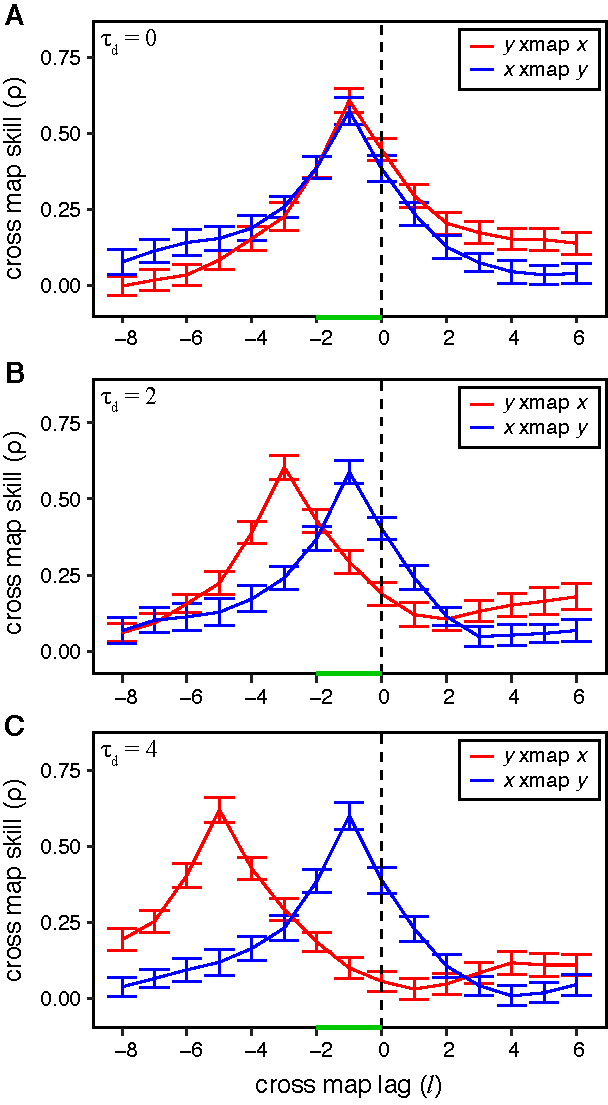
\includegraphics[scale = 0.7]{fig_lag_2sp_delay.pdf}\end{center}
\caption[Model demonstration of causal lags and optimal cross mapping using a 2-species logistic model with bidirectional forcing.]{\textbf{Model demonstration of causal lags and optimal cross mapping using a 2-species logistic model with bidirectional forcing.}\newline
Cross-mapping skill ($\rho$) is shown as a function of cross-mapping lag for three different time delays, $\tau_d$, in the effect of $x$ on $y$. Here, ``$y$ xmap $x$'' refers to using $y$ and its lags to cross map variable $x$ with time lag $l$. (A) With $\tau_d = 0$, both variables respond to each other within a single time-step ($y(t+1)$ is influenced by $x(t)$ and vice-versa), and so the optimal cross map lag occurs at $l = -1$, falling within the embedding vector (green bar) as expected. (B-C) For $\tau_d = 2$ or 4, the effect of $x$ on $y$ is delayed, and so the optimal lag for $y$ cross mapping $x$ (i.e., red line, measuring the effect of $x$ on $y$) shifts back by a corresponding amount, while $x$ cross mapping $y$ is unchanged. Plots show mean cross map skill and standard deviation over 100 random libraries (see Materials and Methods).}
\label{fig_lag_2sp_delay}
\end{figure}

Figure \ref{fig_lag_2sp_delay} shows the results of extended CCM applied to the two-species coupled logistic map (equation \ref{eqn_2sp_delay}). As shown in the first panel (Figure \ref{fig_lag_2sp_delay}A), where causation occurs with an effective delay of 1 time step ($y(t)$ affects $x(t+1)$ and vice-versa), the optimal cross mapping in both directions occurs at a lag of -1. Moreover, as expected, a time delay in the effect of $x$ on $y$ (Figure \ref{fig_lag_2sp_delay}B-C), produces optimal cross mapping (from $y$ to $x$) with a lag corresponding to the degree of time delay. Extending this analysis to systems with random coefficients (see Supplementary Information), the result is robust, with only a few outliers that exhibit optimal cross mapping at different lags (Figure \ref{fig_lag_2sp_delay_rand}). This validates a basic rule of thumb for bidirectional causality: we may reasonably expect optimal cross mapping lags to be negative, and with the magnitude of the lag roughly equal to the time delay of causality.

\begin{figure}[!ht]
\begin{center}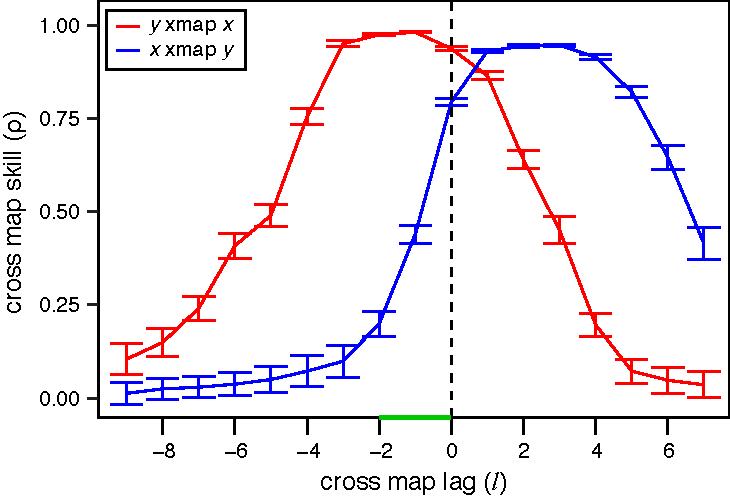
\includegraphics[width=\maxwidth{\textwidth}]{fig_lag_2sp_synch.pdf}\end{center}
\caption[Generalized synchrony in a 2-species logistic model with unidirectional forcing.]{\textbf{Generalized synchrony in a 2-species logistic model with unidirectional forcing.}\newline
In this system, the dynamics of $y$ becomes enslaved to $x$, and so $y$ can be predicted from $x$. Since $x$ affects future values of $y$, $x$ is best able to cross map $y$ forward in time ($l \sim 3 > 0$), whereas cross mapping in the true direction shows optimal prediction for negative time lags ($l \sim -1 < 0$, as in Figure \ref{fig_lag_2sp_delay}). Thus, even though there is cross mapping in both directions, we can use the positive optimal prediction lag to distinguish the direction of causality. As in Figure \ref{fig_lag_2sp_delay}, ``$y$ xmap $x$'' refers to using $y$ and its lags to cross map variable $x$ with time lag $l$; plots show mean cross map skill and standard deviation over 100 random libraries (see Materials and Methods).}
\label{fig_lag_2sp_synch}
\end{figure}

For systems where strong unidirectional causality leads to generalized synchrony (equation \ref{eqn_2sp_synch}), a time delay in the response can be detected using extended convergent cross mapping. Although the response variable ``synchronizes'' to the causal variable, if causality is not instantaneous, the synchronization occurs with some lag that can then be identified using extended convergent cross mapping. In Figure \ref{fig_lag_2sp_synch}, we find that the optimal cross map lag from $y$ to $x$ is negative, as expected; $x$ causes $y$, and so cross map skill is better when estimating the historical influence of $x$ from the response variable $y$. Conversely, the optimal cross map lag from $x$ to $y$ is positive, because even with synchrony, there is no flow of causal information from $y$ to $x$, and so changes in $x$ are not reflected in $y$ until sometime in the future. Thus, the positive lag from $x$ cross mapping $y$ informs us that there is unidirectional causality, even when the interaction is strong enough to result in synchrony. Again, extending this analysis to similar systems with random coefficients (see Supplementary Information), we find that optimal cross map lags can reliably distinguish between generalized synchrony and bidirectional causality (Figure \ref{fig_lag_2sp_synch_rand}).

\begin{figure}[!ht]
\begin{center}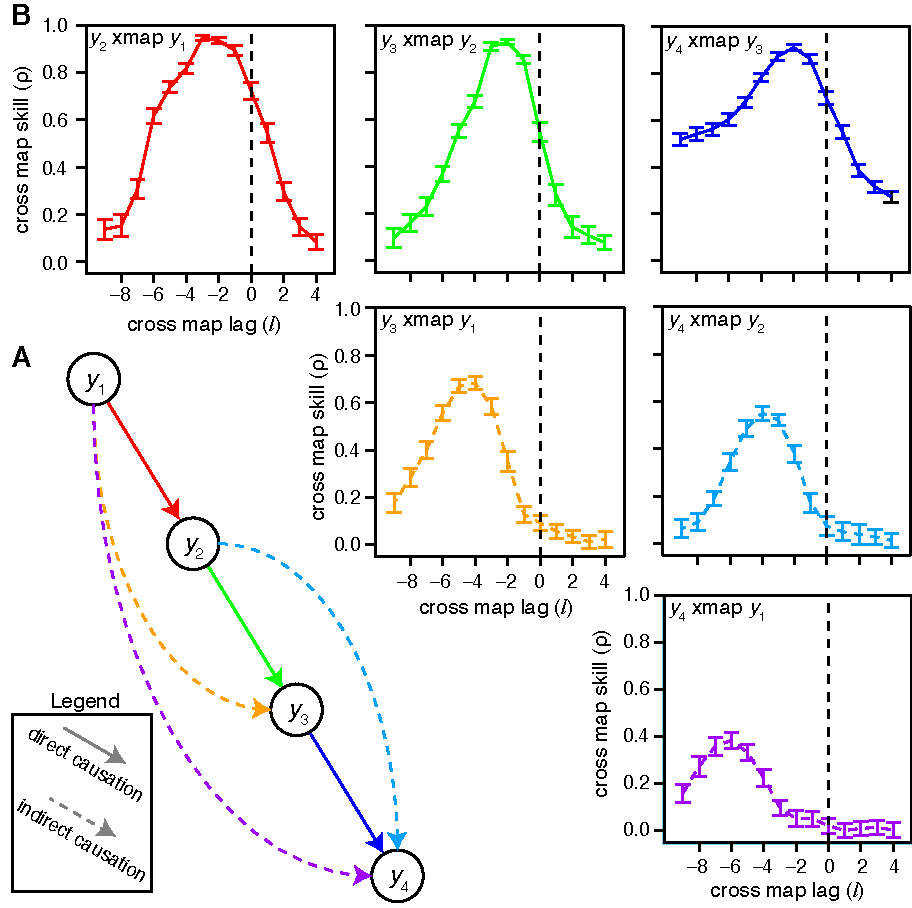
\includegraphics[width=\maxwidth{\textwidth}]{fig_lag_4sp_transitive.pdf}\end{center}
\caption[Direct and indirect causality in a transitive causal chain.]{\textbf{Direct and indirect causality in a transitive causal chain.}\newline
(A) In this system, $y_1$ causes $y_2$ causes $y_3$ causes $y_4$ such that indirect causation from $y_1$ to $y_3$, $y_2$ to $y_4$, and $y_1$ to $y_4$ occurs. (B) Using extended CCM, the direct links (top row) are strongest with the highest cross map skill and the most immediate effects ($l \sim -2$), the indirect links separated by one node (middle row) have moderate cross map skill and somewhat delayed effects ($l \sim -4$), and the indirect link from $y_1$ to $y_4$ (bottom row) is the weakest and with the longest time delay ($l \sim -6$). Here ``$y_i$ xmap $y_j$'' refers to using $y_i$ and its lags to cross map to $y_j$. Plots show mean cross map skill and standard deviation over 100 random libraries (see Materials and Methods).}
\label{fig_lag_4sp_transitive}
\end{figure}

As discussed by Sugihara et al. \cite{Sugihara_2012}, CCM can detect indirect causality that occurs through a transitive causal chain. For example, in the system depicted in Figure \ref{fig_lag_4sp_transitive}A, $y_1$ causes $y_2$ causes $y_3$ causes $y_4$ (equation \ref{eqn_4sp_transitive}). With CCM, we can detect these direct causal connections (e.g., using the cross map from $y_j$ to $y_i$ to infer the effect of $y_i$ on $y_j$). However, there are also indirect effects from $y_1$ to $y_3$, $y_2$ to $y_4$, and $y_1$ to $y_4$. These indirect effects may also appear significant in CCM if coupling is strong enough. To unravel the direct from indirect effects in this system, we can apply extended CCM to identify the optimal cross map lags and optimal cross map skill (Figure \ref{fig_lag_4sp_transitive}B). For the direct links (top row of Figure \ref{fig_lag_4sp_transitive}B), optimal cross mapping occurs with high skill and a small negative lag ($l \sim -2$); for indirect links separated by a single node (middle row of Figure \ref{fig_lag_4sp_transitive}B), optimal cross mapping occurs with moderate skill and a moderate negative lag ($l \sim -4$); and for the indirect link from $y_1$ to $y_4$ (separated by both $y_2$ and $y_3$), optimal cross mapping is weak, and at a large negative lag ($l \sim -6$). When this analysis was repeated for model systems with random coefficients (see Supplementary Information), the differences in optimal cross map lag were relatively robust (Figure \ref{fig_lag_4sp_transitive_rand}). However, cross map skill showed more variance, suggesting that it is a less reliable indicator of direct vs. indirect causation. The outliers are likely a result of stable dynamics (with cross map skill, $\rho$ that reaches 1), since this is a simple model simulated without process error.

\begin{figure}[!ht]
\begin{center}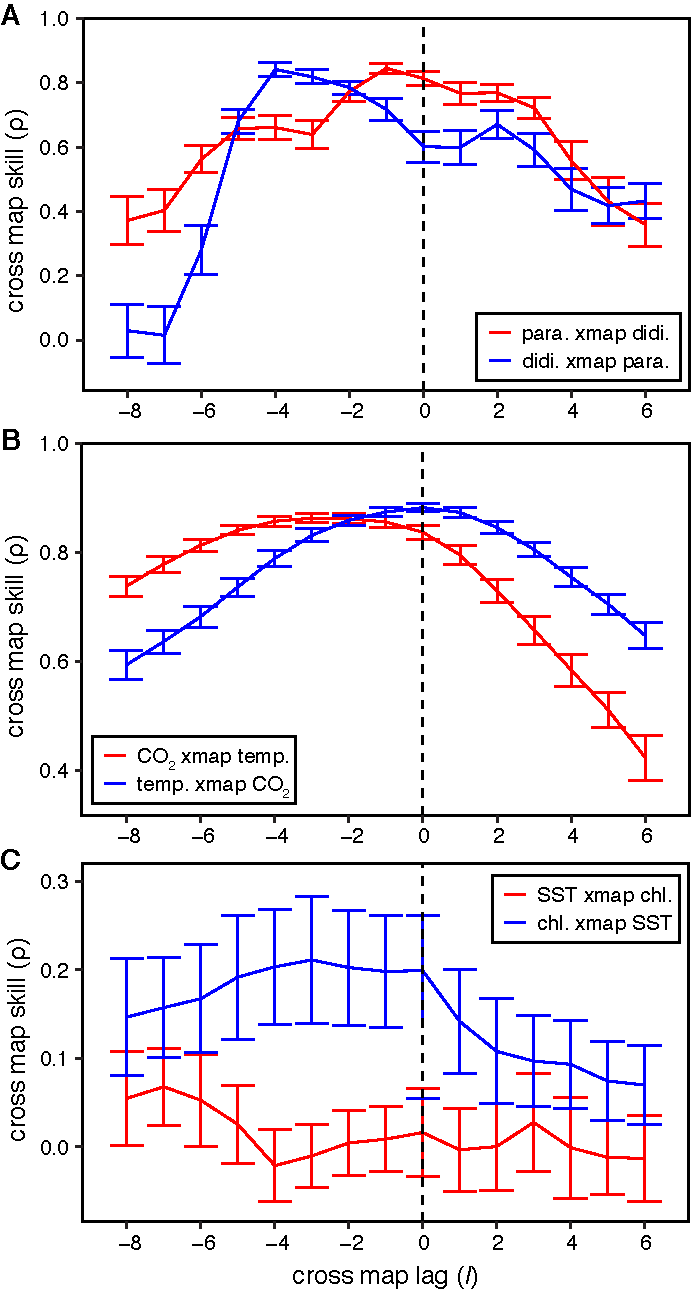
\includegraphics[scale = 0.55]{fig_lag_real_examples.pdf}\end{center}
\label{fig_lag_real_examples}
\caption[Applying extended CCM to real world examples.]{\textbf{Applying extended CCM to real world examples.}\newline
(A) Extended CCM analysis of time series from Veilleux's predator-prey experiment \cite{Veilleux_1976} with \emph{Paramecium aurelia} (prey) and \emph{Didinium nasutum} (predator) reveals bidirectional causality. While the effect of predators on prey (red, ``para. xmap didi.'') is immediate, the effect of prey on predators (blue, ``didi. xmap para.'') shows a distinct lag, as prey ingestion does not instantaneously translate into population growth. (B) Analysis of causality between Earth atmospheric CO$_2$ and temperature using time series data from the Vostok ice core for the previous 412,000 years. As expected CO$_2$ has a nearly instantaneous effect on temperature (blue, ``temp. xmap CO$_2$'') due to the fast-acting greenhouse gas effect, while the influence of temperature on CO$_2$ is much slower, with an optimal CCM lag of $\sim 3000$ years (red, ``CO$_2$ xmap temp.''). (C) Analysis of weekly averages of sea surface temperature (SST) and chlorophyll-a at SIO pier in La Jolla, CA suggests that the effect of SST occurs with a lag of 1-4 weeks (blue, ``chl. xmap SST''). All plots show mean cross map skill and standard deviation over 100 random libraries (see Materials and Methods).}
\end{figure}

\subsection{Veilleux's Paramecium-Didinium Experiment}

Applying extended CCM to the time series of \emph{Paramecium} and \emph{Didinium} from Veilleux's lab experiments \cite{Veilleux_1976}, we confirm the results of Sugihara et al. \cite{Sugihara_2012} showing bidirectional causality. However, whereas Sugihara et al. suggested that the difference in cross mapping predictability (with a lag of 0) was indicative of stronger top-down forcing, our analysis here reveals another layer to the story: considering different lags, we find that cross mapping predictability is roughly equal at optimal lag values (Figure \ref{fig_lag_real_examples}A), suggesting that top-down and bottom-up effects are equally important. We do note that the optimal cross mapping lag does depend on the interaction: an optimal lag of -1 for the \emph{Paramecium} cross mapping \emph{Didinium} direction suggests that \emph{Paramecium} respond quickly to changes in \emph{Didinium} abundance. However, an optimal lag of -4 for the \emph{Didinium} cross mapping \emph{Paramecium} direction suggests that \emph{Didinium} respond more slowly to changes in \emph{Paramecium} abundance. These results are consistent with the ecological context of this system \cite{Li_2013}: the prey (\emph{Paramecium}) respond quickly to predators (\emph{Didinium}) because predator-induced mortality has an immediate (negative) effect on the abundance of prey, whereas the abundance of predators (\emph{Didinium}) responds more slowly to prey (\emph{Paramecium}), because of the time delay in converting food into new individuals.

\subsection{Vostok Ice Core}

Figure \ref{fig_lag_real_examples}B shows the application of extended convergent cross mapping to time series of CO$_2$ and temperature reconstructed from the Vostok ice core \cite{Petit_1999}. Here, we detect bidirectional causality (the optimal cross mapping lag is negative in both directions), suggesting that there is a positive feedback in the Earth's climate system between temperature and greenhouse gases. Notably, the optimal lag in the temperature to CO$_2$ direction matches current scientific knowledge that greenhouse gases have a rapid effect on temperature (faster than the 1000-year timescale of the data), while the influence of global temperature on greenhouse gases likely occurs through slower mechanisms (e.g., increased plant respiration at higher temperatures \cite{Cramer_2001}, release of greenhouse gases from terrestrial \cite{Schuur_2009} or marine ecosystems \cite{Archer_2009}). A detailed analysis of this system appears in van Nes et al. \cite{Nes_2015}.

\subsection{Southern California Bight}

In Figure \ref{fig_lag_real_examples}C, we show the results of extended CCM applied to long-term time series of chlorophyll-a and sea surface temperature measured at the Scripps Institution of Oceanography pier. As expected, there is no effect of chlorophyll-a on SST (red line). However, we do identify a causal influence of SST on chlorophyll-a, suggesting that the physical environment plays a role in determining phytoplankton abundances (which are proxied by concentrations of chlorophyll-a). Moreover, optimal cross mapping occurs with a lag of 3 weeks, suggesting that the physical drivers of algae populations act with a lag of several weeks. Ideally, if other causal drivers show similar time delays in their effects, then it may be possible to produce models that can forecast events such as algal blooms several weeks in advance!

\subsection{Stochastic Drivers}

We note that in certain systems, especially those with stochastic drivers that contain unique information, Granger causality may correctly identify causal interactions. Indeed, Granger causality has been successful when applied to system consisting solely of stochastic components. However, in situations where both cause and effect have deterministic dynamics, causal information cannot be isolated from amongst the affected variables, and alternative methods, such as CCM must therefore be used.

\subsection{Final Remarks}

Here, we have shown that explicitly considering time lags when applying convergent cross mapping can be a valuable tool beyond the simple test of whether two variables are causally related. Although this general approach has been explored elsewhere \cite{Schumacher_2015}, here we show how the CCM framework can be directly extended to account for temporal delays. As demonstrated in our model simulations, CCM can now distinguish synchrony induced by strong unidirectional forcing from true bidirectional causation (Figure \ref{fig_lag_2sp_synch}), as well as order nodes in transitive causal chains that produce direct and indirect causal links (Figure \ref{fig_lag_4sp_transitive}). 

In addition, we show how identification of time delays can clarify our understanding of the causal effects, which can be valuable in producing a more detailed and mechanistic description of causal dynamics in real systems. For example, knowing the approximate time delay of causal interactions can be important when forecasting future events -- although in general, a single time series contains all necessary dynamic information, this will not be the case when stochastic drivers are influencing the dynamics. Since the stochastic driver has unique information, it must be explicitly included at the appropriate lag for optimal predictability (see ref. \cite{Deyle_2013, Ye_2015} for examples). Moreover, understanding the delayed effect of external drivers will be important in management scenarios, as knowing when to expect the system to respond to interventions or manipulations will guide future management actions.

\section{Methods}

\subsection{Convergent Cross Mapping}

The basic principle of cross mapping involves reconstructing system states from two time series variables and then quantifying the correspondence between them using nearest neighbor forecasting \cite{Sugihara_1990}. Reconstruction is done using the method of time delay embedding: with the system state represented using successive lags of a single time series \cite{Takens_1981, Packard_1980}. For example, given a time series $\{y(t)\}$, an $E$-dimensional reconstruction uses $E$ successive lags of $y$, each separated by a time step $\tau$: $\langle y(t), y(t-\tau), \dots, y(t - (E-1)\tau) \rangle$.

We note that the optimal value of the embedding dimension $E$ depends on several factors, including system complexity, time series length, and noise. In the case of model systems, the number of interacting variables is known exactly and was used to select $E$. In the remaining cases, the value of $E$ was determined empirically by applying simplex projection \cite{Sugihara_1990} to the individual time series and choosing the optimal $E$. Since most time series were not overly sampled in time, we fixed $\tau = 1$ for all systems. 

In the case of a system where $x$ causes $y$, Takens' Theorem \cite{Takens_1981} implies that there should be a correspondence between the state $\vec{y}(t)$ and the contemporaneous state $\vec{x}(t)$. Convergent cross mapping (CCM \cite{Sugihara_2012}) quantifies this relationship using simplex projection (a nearest-neighbor forecasting method, see ref. \cite{Sugihara_1990} for details) to estimate the scalar value $x(t)$ from the reconstructed vector $\vec{y}(t)$ (see ref. \cite{Sugihara_2012} and Movie S3 for details). Although different performance metrics are possible, here we use Pearson's correlation coefficient between the estimated and observed values of $x(t)$ as an indicator of ``cross map skill''.

We note that, in general, one may compute a function that maps from $\vec{y}(s)$ to the entire vector $\vec{x}(s)$ as opposed to just the scalar value $x(s)$ \cite{Schiff_1996, Ma_2014}. However, doing so can decrease the sensitivity of the cross mapping idea, because the errors are no longer scalar values, but $E$-dimensional vectors, for which common distance metrics can become meaningless \cite{Aggarwal_2001}. Moreover, by estimating entire vectors, we limit the capability to use cross mapping to analyze time delays in the effect of $x$ on $y$, which we show here can be informative in an extended version of CCM (see below).

\subsection{Extended Convergent Cross Mapping}

\begin{figure}[!ht]
\begin{center}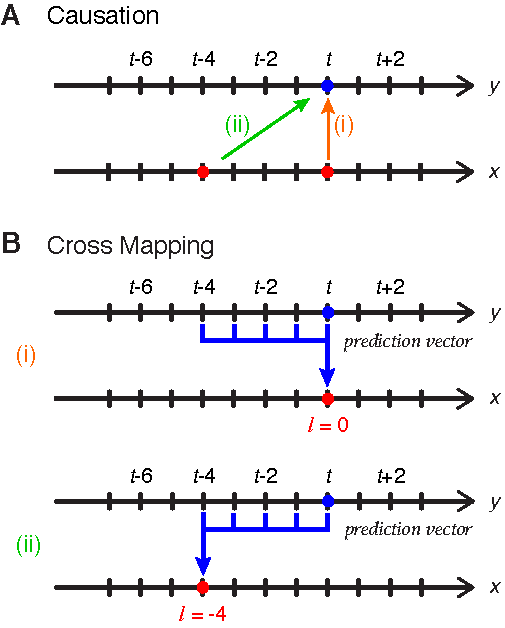
\includegraphics[width=\maxwidth{\textwidth}]{fig_lag_extended_ccm.pdf}\end{center}
\caption[Effect of time delays on cross mapping.]{\textbf{Effect of time delays on cross mapping.}\newline
Panel A shows causation for two cases: (i) no time delay in the effect of $x$ on $y$ (i.e., $y$ responds instantaneously to $x$), and (ii) $y$ responds to $x$ with a time delay of 4 (time steps). Panel B shows (i) cross mapping with $l = 0$, equivalent to the original formulation by Sugihara et al. \cite{Sugihara_2012} and (ii) cross mapping with $l = -4$, which may be expected to be better than $l = 0$ when $x$ acts on $y$ with some time delay.}
\label{fig_lag_real_examples}
\end{figure}

Standard cross mapping when $x$ causes $y$ (Figure \ref{fig_lag_real_examples}A) computes the predictability of $x(t)$ from the $E$-dimensional reconstruction $\vec{y}(t) = \langle y(t), y(t-\tau), \dots, y(t - (E-1)\tau) \rangle$ (Figure \ref{fig_lag_real_examples}B.i). However, the general theory of CCM \cite{Sugihara_2012}, based on generalizations of Takens' Theorem \cite{Sauer_1991, Deyle_2011}, suggests that we should also be able to cross map from $\vec{y}(t)$ to $x(t+l)$, for any reasonable lag value of $l$, since the variable $x(t+l)$ is simply another observation function of the system. In fact, if $x$ acts on $y$ with some time delay (Figure \ref{fig_lag_real_examples}A.ii), then the current state of the system, $\vec{y}(t)$, will better predict the past values of $x$ (Figure \ref{fig_lag_real_examples}B.ii).

In general, we note that optimal predictability may be expected to occur for some $l < 0$, even if $y$ responds instantaneously to $x$ \cite{Casdagli_1991}. In other words, the state of the system at a time $t$ is often best estimated from a reconstruction that includes both past and future values. This phenomenon occurs because information in a dynamic system can be thought of as propagating both forwards and backwards through time. In other words, knowing the exact value of variable $x$ at time $t$ restricts the likely set of possible futures (the value at time $t+1$) as well as the likely set of possible pasts (the state at time $t-1$). Furthermore, the exact amount of information contained in past (and future) values of $x$ is determined by the rate at which predictability decreases when we forecast further into the future (or past). Consequently, this means the most information about the current system state occurs with a combination of forward and backward lags \cite{Casdagli_1991}: a time-centered embedding that balances positive and negative lags: $\langle y(t), y(t-\tau), y(t+\tau), \dots y(t-(E-1)\tau/2), y(t+(E-1)\tau/2) \rangle$. In the context of extended CCM, this then suggests that the optimal lag will occur in the middle of the prediction vector: $l = (E-1)\tau/2$. In reality, however, the optimal lag will vary from system to system; so while the ``middle of the vector'' is a useful heuristic, optimal cross mapping at any lag that lies within the embedding vector, $-(E-1)\tau \le l \le 0$, is consistent with an influence of $x$ on $y$ with no time delay.

\subsection{Two-Species Model System with Bidirectional Causality}

We first consider a simple model system consisting of 2 coupled logistic difference equations:
\begin{align}
\label{eqn_2sp_delay}
\begin{split}
x(t+1) &= x(t) \left[3.78 - 3.78 x(t) - 0.07 y(t)\right]\\
y(t+1) &= y(t) \left[3.77 - 3.77 y(t) - 0.08 x(t-\tau_d)\right]
\end{split}
\end{align}
where $\tau_d$ is the time delay for the effect of $x$ on $y$. The system is initialized as $x(1) = 0.2$ and $y(1) = 0.4$, and run for 3000 time steps, with different values for the time delay: $\tau_d = 0$, $\tau_d = 2$, and $\tau_d = 4$. Using extended CCM, we analyze this system using $E = 2$, $\tau = 1$, selecting 100 random libraries of 200 vectors over time points 101-2000, and computing cross map skill for time points 2001-3000.

\subsection{Two-Species Model System with Synchrony}

We also examine a modified form of the above system with causality from $x$ to $y$ only:
\begin{align}
\label{eqn_2sp_synch}
\begin{split}
x(t+1) &= x(t) \left[3.8 - 3.8 x(t)\right]\\
y(t+1) &= y(t) \left[3.1 - 3.1 y(t) - 0.8 x(t)\right]
\end{split}
\end{align}
As above, the system is initialized as $x(1) = 0.2$ and $y(1) = 0.4$, and run for 1000 time steps. Because of the strong forcing of $x$ on $y$, the dynamics of $y$ are entrained to those of $x$ (i.e., ``generalized synchrony'' \cite{Rulkov_1995}). Thus, we apply extended CCM to identify the optimal cross map lag and distinguish this case from the case of bidirectional causality. In this system, we also use $E = 2$, $\tau = 1$, selecting random libraries of 200 vectors over time points 101-2000, and computing cross map skill for time points 2001-3000.

\subsection{Four-Species Model System}

To demonstrate extended CCM in systems with indirect causality (as a result of a transitive causal chain), we consider a 4-species model system. The system is initialized as $y_1(1) = y_2(1) = y_3(1) = y_4(1) = 0.4$, and evolves according to:
\begin{align}
\label{eqn_4sp_transitive}
\begin{split}
y_1(t+1) &= y_1(t) \left[3.9 - 3.9 y_1(t)\right]\\
y_2(t+1) &= y_2(t) \left[3.6 - 0.4 y_1(t) - 3.6 y_2(t)\right]\\
y_3(t+1) &= y_3(t) \left[3.6 - 0.4 y_2(t) - 3.6 y_3(t)\right]\\
y_4(t+1) &= y_4(t) \left[3.8 - 0.35 y_3(t) - 3.8 y_4(t)\right]
\end{split}
\end{align}

Although the only direct causal links are from $y_1$ to $y_2$, from $y_2$ to $y_3$, and from $y_3$ to $y_4$, this creates a transitive chain of causality, such that there is an indirect influence of $y_1$ on $y_3$, from $y_2$ to $y_4$, and from $y_1$ to $y_4$ (Figure \ref{fig_lag_4sp_transitive}a). Thus, we apply extended CCM with $E = 4$ and $\tau = 1$ to distinguish between direct and indirect causation. For each pair, we sample 100 random libraries of size 200 from time points 101-1000 and compute the cross map skill for time points 2001-3000.

\subsection{\emph{Paramecium}-\emph{Didinium} Predator-Prey System}

We examine causality in a classical predator-prey system, the \emph{Paramecium}-\emph{Didinium} protozoan system using experimental time series from Veilleux \cite{Veilleux_1976}, who refined earlier work from Gause \cite{Gause_1935} and Luckinbill \cite{Luckinbill_1973} to establish sustained oscillations. The data we used came from dataset 11a, and can be found at: \url{http://robjhyndman.com/tsdldata/data/veilleux.dat}. CCM analysis was done using $E = 3$, and $\tau = 1$. Libraries were bootstrap samples over all 71 points of data, and cross map skill was computed using leave-one-out cross-validation over the same,

\subsection{Vostok Ice Core}

Time series for historical Earth temperature and atmospheric CO$_2$ concentration were based on reconstructions from the Vostok ice core \cite{Veilleux_1976} and span $\sim$410,000 years. To produce time series with regular intervals, we linearly interpolated the raw reconstructions to obtain estimates of temperature and CO$_2$ spaced every 1000 years. CCM analysis was done by sampling 100 random libraries of size 100 and predicting over all 412 points of data, using leave-one-out cross-validation, $E = 4$, and $\tau = 1$.

\subsection{Scripps Pier Time Series}

Chlorophyll-a data came from measurements collected twice weekly at the end of the Scripps Institution of Oceanography's pier (SIO Pier) as part of the Southern California Coastal Ocean Observing System, Harmful Algal Bloom Monitoring Program. Sea Surface Temperature (SST) was sampled daily as part of the Shore Stations Program, also at SIO Pier. Because of irregular sampling, we processed the data to construct weekly time series for the period June 30, 2008 to May 26, 2014. Extended CCM was then applied to investigate the relationship between SST and chlorophyll-a using $E = 4$ and $\tau = 1$ (corresponding to 1 week) and sampling 100 random libraries of size 100 and predicting over all 306 points of data.

\section{Supplementary Information}

\subsection{Two-Species Model System with Bidirectional Causality}

\begin{figure}[!ht]
\begin{center}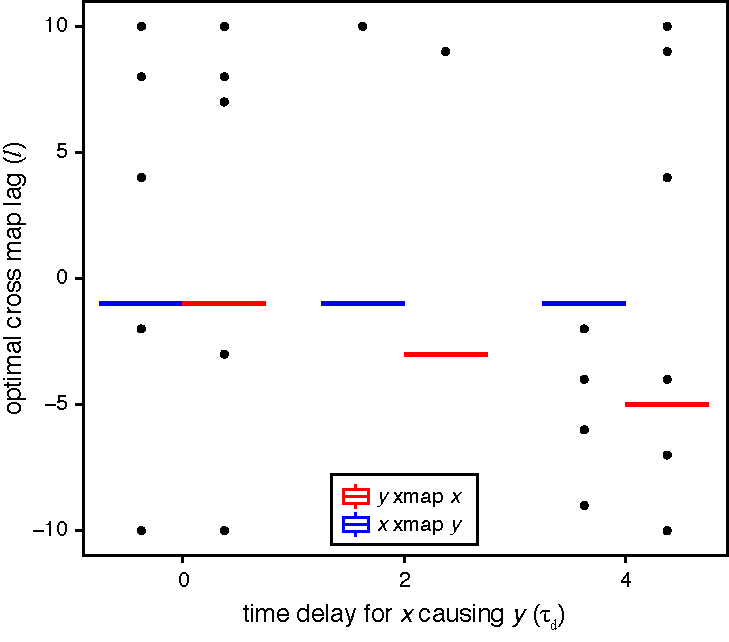
\includegraphics{fig_lag_2sp_delay_rand.pdf}\end{center}
\caption[Robustness of extended CCM in the 2-species logistic model with bidirectional forcing.]{\textbf{Robustness of extended CCM in the 2-species logistic model with bidirectional forcing.}\newline
Boxplots of optimal cross map lag ($l$) are shown for 500 random simulations of the 2-species logistic model with bidirectional causality and with three different time delays, $\tau_d$. Except for a few outliers, the optimal cross map lag when using $x$ to cross map $y$ (blue, ``$x$ xmap $y$'') is -1, as would be expected, because $x$ responds to $y$ within a single time step. In the opposite direction, a larger time delay ($\tau_d$) in the effect of $x$ on $y$ results in larger negative values for the optimal cross map lag when using $y$ to cross map $x$ (red, ``$y$ xmap $x$'')}
\label{fig_lag_2sp_delay_rand}
\end{figure}

We generalize the simple model system consisting of 2 coupled logistic difference equations as follows:
\begin{align}
\label{eqn_2sp_delay_rand}
\begin{split}
x(t+1) &= x(t) \left[R_x - R_x x(t) - A_{xy} y(t)\right]\\
y(t+1) &= y(t) \left[R_y - R_y y(t) - A_{yx} x(t-\tau_d)\right]
\end{split}
\end{align}

where $\tau_d$ is the time delay for the effect of $x$ on $y$. For each simulation run, we sample a new fixed value for the growth rates $R_x$ and $R_y$ from the uniform distribution $(3.7, 3.9)$, as well as new values for the interaction coefficients $A_{xy}$ and $A_{yx}$ from the uniform distribution $(0.05, 0.1)$. In addition each simulation is initialized with random starting points with $x(1)$ and $y(1)$ drawn from the uniform distribution $(0.01, 0.99)$, and run for 3000 time steps. For each of the different values for the time delay: $\tau_d = 0$, $\tau_d = 2$, and $\tau_d = 4$, we ran a total of 500 simulations (when populations reached negative values or increased beyond carrying capacity, we sampled new coefficients and re-ran the simulation). Using extended CCM, we analyze each simulation using $E = 2$, $\tau = 1$, selecting a random library of 200 vectors over time points 101-2000, and computing cross map skill for time points 2001-3000.

The results are depicted in Figure \ref{fig_lag_2sp_delay_rand}, with boxplots for the value of the cross map lag ($l$) that gives the highest cross map skill ($\rho$). Because nearly all simulations had identical values for the optimal cross map lag ($l$), the boxplots are depicted as straight lines with just a few outliers. As expected, ``$y$ xmap $x$'' (red), depicting the causal effect of $y$ on $x$ has an optimal cross map lag of $l = -1$, because $y$ affects $x$ with a lag of 1 time step ($y(t)$ influences $x(t+1)$). Conversely, the optimal cross map lag for ``$x$ xmap $y$'' (blue) changes depending on $\tau_d$; this is also expected since $\tau_d$ describes the time delay in the response of $y$ to $x$. In fact, the optimal cross map lag for ``$x$ xmap $y$'' appears to accurately recover the time delay parameter $\tau_d$: for example, the optimal $l$ is nearly always -3 when $\tau_d = 2$ (meaning $x(t)$ influences $y(t+3)$ and therefore it takes 3 time steps for $y$ to respond to $x$).

\subsection{Two-Species Model System with Synchrony}

\begin{figure}[!ht]
\begin{center}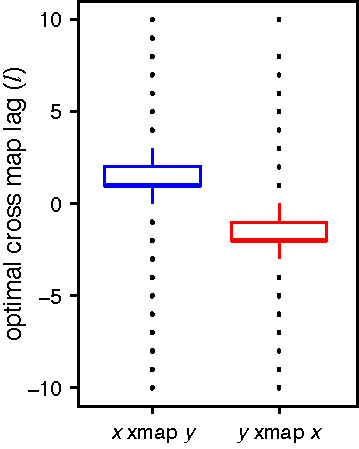
\includegraphics{fig_lag_2sp_synch_rand.pdf}\end{center}
\caption[Robustness of extended CCM in the 2-species logistic model with generalized synchrony.]{\textbf{Robustness of extended CCM in the 2-species logistic model with generalized synchrony.}\newline
Boxplots of optimal cross map lag ($l$) are shown for 500 random simulations of the 2-species logistic model with unidirectional causality producing generalized synchrony. Except for a few outliers, the optimal cross map lag when using $y$ to cross map $x$ (red, ``$y$ xmap $x$'') is negative, and positive in the opposite direction (blue, ``$x$ xmap $y$''). This is expected, because $x$ has a true causal influence on future values of $y$, meaning $y$ is better at cross mapping to past values of $x$; conversely, the lack of an actual effect of $y$ on $x$, but rather ``generalized synchrony'' means that $x$ is better at cross mapping future values of $y$.}
\label{fig_lag_2sp_synch_rand}
\end{figure}

We also generalize the modified form of the above system that produces synchrony with strong forcing from x to y only:

\begin{align}
\label{eqn_2sp_synch_rand}
\begin{split}
x(t+1) &= x(t) \left[R_x - R_x x(t)\right]\\
y(t+1) &= y(t) \left[R_y - R_y y(t) - A_{yx} x(t)\right]
\end{split}
\end{align}

For each simulation, $R_x$ is sampled from the uniform distribution $(3.7, 3.9)$, $R_y$ is sampled from the uniform distribution $(2.5, 3.2)$, and $A_{yx}$ is sampled from the uniform distribution $(0.7, 0.9)$. As above, the system is initialized with random starting points with $x(1)$ and $y(1)$ drawn from the uniform distribution $(0.01, 0.99)$, and run for 3000 time steps. We ran a total of 500 simulations (when populations reached negative values or increased beyond carrying capacity, we sampled new coefficients and re-ran the simulation). Using extended CCM, we analyze each simulation using $E = 2$, $\tau = 1$, selecting a random library of 200 vectors over time points 101-2000, and computing cross map skill for time points 2001-3000.

Results for the ``generalized synchrony'' model are shown in Figure \ref{fig_lag_2sp_synch_rand}, with boxplots showing the value of the cross map lag ($l$) that gives the highest cross map skill ($\rho$). Again, we see that the optimal cross map lag ($l$) is generally negative in the direction of true causality (red, ``$y$ xmap $x$'') and positive in the direction of synchrony (blue, ``$x$ xmap $y$''). 

\subsection{Four-Species Model System}

To test the robustness of extended CCM in distinguishing between direct and indirect causality, we generalize the 4-species model system with a transitive causal chain:

\begin{align}
\label{eqn_4sp_transitive_rand}
\begin{split}
y_1(t+1) &= y_1(t) \left[R_1 - R_1 y_1(t)\right]\\
y_2(t+1) &= y_2(t) \left[R_2 - A_{21} y_1(t) - R_2 y_2(t)\right]\\
y_3(t+1) &= y_3(t) \left[R_3 - A_{32} y_2(t) - R_3 y_3(t)\right]\\
y_4(t+1) &= y_4(t) \left[R_4 - A_{43} y_3(t) - R_4 y_4(t)\right]
\end{split}
\end{align}

For each simulation, the growth parameters are sampled as follows: $R_1$ is drawn from the uniform distribution $(3.8, 4.0)$, $R_2$ and $R_3$ are both drawn from the uniform distribution $(3.5, 3.7)$, and $R_4$ is drawn from the uniform distribution $(3.7, 3.9)$. The interaction parameters $A_{21}$, $A_{32}$, and $A_{43}$ are all drawn from the uniform distribution $(0.3, 0.5)$. As above, the system is initialized with random starting points with each $y_i(1)$ drawn from the uniform distribution $(0.01, 0.99)$, and run for 3000 time steps. We ran a total of 500 simulations (when populations reached negative values or increased beyond carrying capacity, we sampled new coefficients and re-ran the simulation). Using extended CCM, we analyze each simulation using $E = 4$, $\tau = 1$, selecting a random library of 200 vectors over time points 101-2000, and computing cross map skill for time points 2001-3000.

\begin{figure}[!ht]
\begin{center}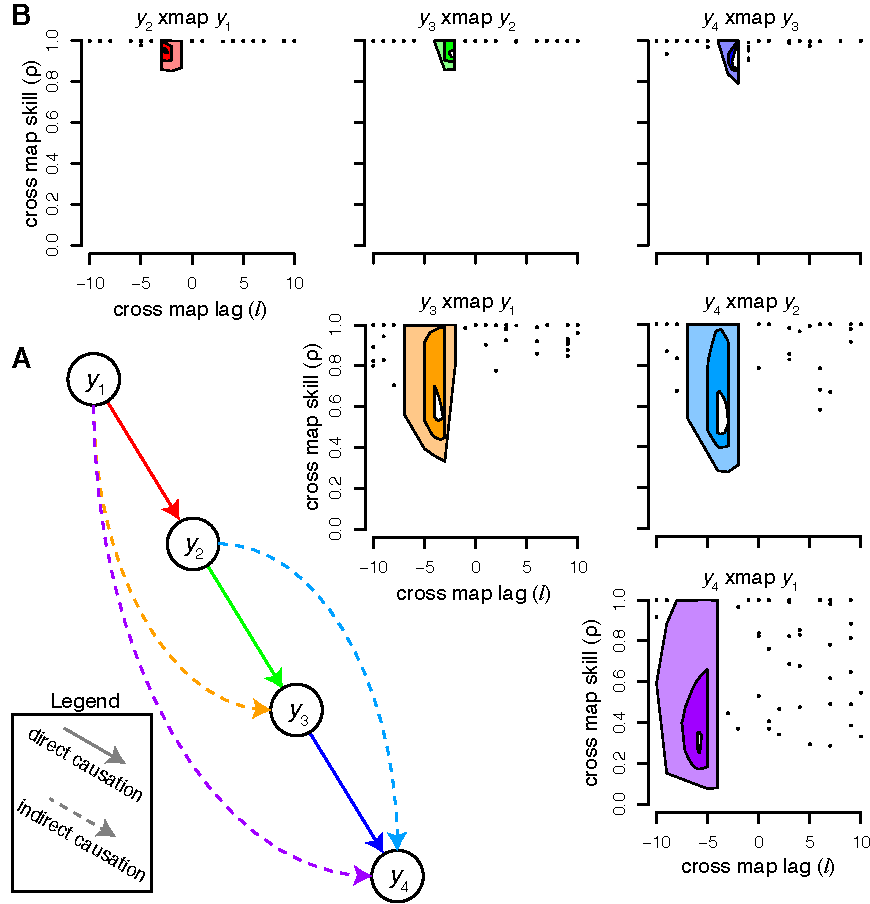
\includegraphics[scale = 0.9]{fig_lag_4sp_transitive_rand.pdf}\end{center}
\label{fig_lag_4sp_transitive_rand}
\caption[Robustness of extended CCM for distinguishing direct and indirect causality in a transitive causal chain.]{\textbf{Robustness of extended CCM for distinguishing direct and indirect causality in a transitive causal chain.}\newline
(A) In this system, $y_1$ causes $y_2$ causes $y_3$ causes $y_4$ such that indirect causation from $y_1$ to $y_3$, $y_2$ to $y_4$, and $y_1$ to $y_4$ occurs. (B) Bagplots show the optimal cross map lag ($l$) and corresponding cross map skill ($\rho$) for 500 random simulations of this system. The white central area depicts the 95\% confidence interval for the median value, while the darker colored region is the ``bag'' containing the central 50\% of points (i.e., similar to an interquartile range), and the lighter colored region is the loop with area 3 times the size of the bag, as described in \cite{Rousseeuw_1999}. The direct links (top row) are strongest with the highest cross map skill and the most immediate effects ($l \sim -2$), while the indirect links separated by one node (middle row) have moderate cross map skill and somewhat delayed effects ($l \sim -4$), and the indirect link from $y_1$ to $y_4$ (bottom row) is the weakest and with the longest time delay ($l \sim -6$)}
\end{figure}

Results for this analysis are shown in Figure \ref{fig_lag_4sp_transitive_rand}, with bagplots \cite{Rousseeuw_1999} depicting the bivariate boxplots for the optimal cross map lags $l$) and corresponding cross map skill ($\rho$). As in Figure \ref{fig_lag_4sp_transitive}, the top row of panel b shows that the optimal cross map lags are close to 0 and show high cross map skill, as would be expected for these direct interactions. In contrast, the indirect interactions generally have optimal cross map lags that are more negative, and lower cross map skill, with the most indirect interaction (from $y_1$ to $y_4$, identified using $y_4$ xmap $y_1$) showing the most negative cross map lag and the lowest cross map skill. We note that the variance in cross map skill is quite high, indicating that it may not be as useful in separating direct from indirect interactions in real systems, whereas cross map lag shows clearer separation.

\section{Acknowledgments}
This research is supported by Department of Defense, Strategic Environment Research and Development Program RC-2509 (GS, ERD, HY), Lenfest Ocean Program \#00028335 (GS), National Science Foundation Grant No. DEB-1020372 (GS, HY), NSF-NOAA Comparative Analysis of Marine Ecosystem Organization (CAMEO) program Grant NA08OAR4320894/CAMEO (GS), National Science Foundation Graduate Research Fellowships (ERD, HY), Environmental Protection Agency Science to Achieve Results Fellowship (ERD), European Research Council Advanced Grant (LJG, awarded to Jordi Bascompte), the Sugihara Family Trust (GS), the Deutsche Bank-Jameson Complexity Studies Fund (GS), and the McQuown Chair in Natural Science (GS).

Chapter \ref{chap_ccm_time_delays}, in full, is a reprint of material published by Nature Publishing Group as: Hao Ye, Ethan R. Deyle, Luis J. Gilarranz, and George Sugihara. (2015) Distinguishing time-delayed causal interactions using convergent cross mapping. \emph{Scientific Reports} 5: 14750. The dissertation author was the primary investigator and author of this paper.